% !TEX TS-program = pdflatex
% !TEX encoding = UTF-8 Unicode

% This is a simple template for a LaTeX document using the "article" class.
% See "book", "report", "letter" for other types of document.

\documentclass[20pt]{article} % use larger type; default would be 10pt

\usepackage[utf8]{inputenc} % set input encoding (not needed with XeLaTeX)

%%% Examples of Article customizations
% These packages are optional, depending whether you want the features they provide.
% See the LaTeX Companion or other references for full information.

%%% PAGE DIMENSIONS
\usepackage{geometry} % to change the page dimensions
\geometry{a4paper} % or letterpaper (US) or a5paper or....
% \geometry{margin=2in} % for example, change the margins to 2 inches all round
% \geometry{landscape} % set up the page for landscape
%   read geometry.pdf for detailed page layout information

\usepackage{graphicx} % support the \includegraphics command and options

% \usepackage[parfill]{parskip} % Activate to begin paragraphs with an empty line rather than an indent

%%% PACKAGES
\usepackage{booktabs} % for much better looking tables
\usepackage{array} % for better arrays (eg matrices) in maths
\usepackage{paralist} % very flexible & customisable lists (eg. enumerate/itemize, etc.)
\usepackage{verbatim} % adds environment for commenting out blocks of text & for better verbatim
%\usepackage{subfig} % make it possible to include more than one captioned figure/table in a single float
\usepackage{mathtools}
\usepackage{graphicx} % supports images in latex
% These packages are all incorporated in the memoir class to one degree or another...

\usepackage{graphicx}
\usepackage{subcaption}

%%% Other stuff
\DeclarePairedDelimiter\ceil{\lceil}{\rceil}
\DeclarePairedDelimiter\floor{\lfloor}{\rfloor}

%%% HEADERS & FOOTERS
\usepackage{fancyhdr} % This should be set AFTER setting up the page geometry
\pagestyle{fancy} % options: empty , plain , fancy
\renewcommand{\headrulewidth}{0pt} % customise the layout...
\lhead{}\chead{}\rhead{}
\lfoot{}\cfoot{\thepage}\rfoot{}

%%% SECTION TITLE APPEARANCE
\usepackage{sectsty}
\allsectionsfont{\sffamily\mdseries\upshape} % (See the fntguide.pdf for font help)
% (This matches ConTeXt defaults)

%%% ToC (table of contents) APPEARANCE
\usepackage[nottoc,notlof,notlot]{tocbibind} % Put the bibliography in the ToC
\usepackage[titles,subfigure]{tocloft} % Alter the style of the Table of Contents
\renewcommand{\cftsecfont}{\rmfamily\mdseries\upshape}
\renewcommand{\cftsecpagefont}{\rmfamily\mdseries\upshape} % No bold!

%%% graphics path
\usepackage{amsmath}
\usepackage{listings}
%\begin{lstlisting}[language=java]
%\end{lstlisting}



%%% END Article customizations

%%% nice things to keep around
%\begin{figure}[!htbp]
%  	\centering
%   	\begin{subfigure}[p]{0.5\linewidth}
%    	\includegraphics[width=\linewidth]{}
%   	\end{subfigure}
%\end{figure} 

% \noindent\rule{2cm}{0.4pt} 
%%% puts a small horizontal line

% \mathcal{O} 
%%% big O notation

% \begin{table}[!htbp]
% \caption{Forward slash.}
% \[\begin{array}{c|ccccc} 
% abc/def & 1 & 2 & 3 & 4 & 5\\
% \hline
% 1 & a & b & c & d & e\\
% 2 & f & g & h & i & j\\
% 3 & k & l & m & n & o\\
% \end{array}\]
% \end{table}

%%% The "real" document content comes below...

\title{Computational Statistics Final}
\author{Liam Dillingham}
%\date{} % Activate to display a given date or no date (if empty),
         % otherwise the current date is printed 

\begin{document}
\maketitle

\section{R Code for Data Preprocessing}
\begin{lstlisting}[language=R]
# Biplot great for visualization
library(devtools)
install_github("vqv/ggbiplot")
library(ggbiplot)

library(ISLR)
nci.labs=NCI60$labs  ## NCI data
nci.data=NCI60$data ## Labels
dim(nci.data)

# Scale data to have mean=0 and sd=1 (each gene on same scale)
sd.data = scale(nci.data) #

nci.pca = prcomp(nci.data, center = T, scale. = T)
summary(nci.pca)

write.csv(nci.pca$x, file = "nci60.csv", row.names = F)
\end{lstlisting}

\section{Python Code}
\begin{lstlisting}[language=python]
import pandas as pd
import numpy as np

import matplotlib as mpl 
import matplotlib.pyplot as plt 
import seaborn as sns

from sklearn.cluster import SpectralClustering, AgglomerativeClustering, DBSCAN, KMeans
from sklearn.manifold import TSNE, MDS

plt.style.use('classic')

# cancer_data = pd.read_csv('./nci60.csv') # data is already standardized
cancer_data = pd.read_csv('./nci60.csv')

# We determined that we need 39 PCs to get >85% of the variance
pcs = []
for i in range(39):
    pcs.append('PC{}'.format(i+1))
cancer_subset = cancer_data[pcs]

sum_of_squared_distances = []
K = range(1,30)
for k in K:
    km = KMeans(n_clusters=k, n_init = 50, random_state = 0)
    km = km.fit(cancer_subset)
    sum_of_squared_distances.append(km.inertia_)

plt.plot(K, sum_of_squared_distances, 'bx-')
plt.xlabel('k')
plt.ylabel('Sum_of_squared_distances')
plt.title('Elbow Method For Optimal k')
plt.show()
\end{lstlisting}


\begin{figure}[!htbp]
  	\centering
   	\begin{subfigure}[!htbp]{0.7\linewidth}
    	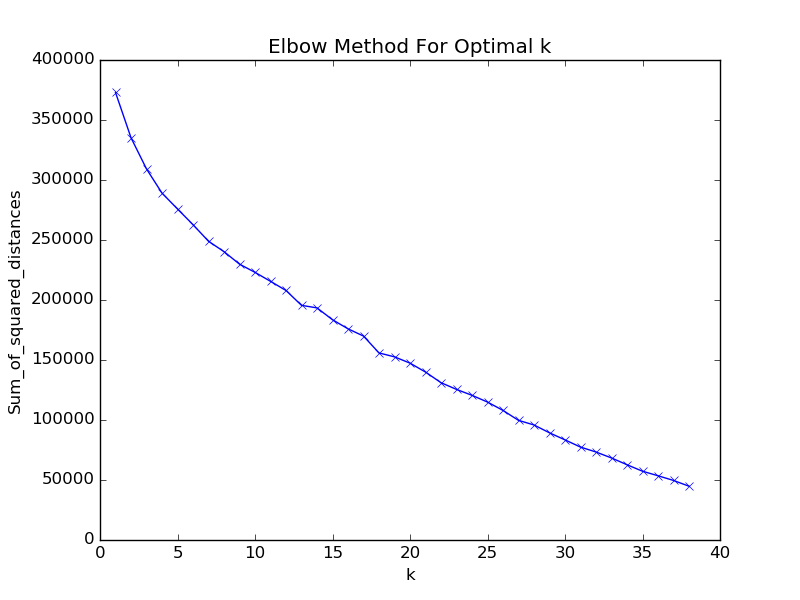
\includegraphics[width=\linewidth]{./figures/kmax50.png}
	\caption{Optimal $k$ for maximum $k=50$}
   	\end{subfigure}
   	\begin{subfigure}[!htbp]{0.7\linewidth}
    	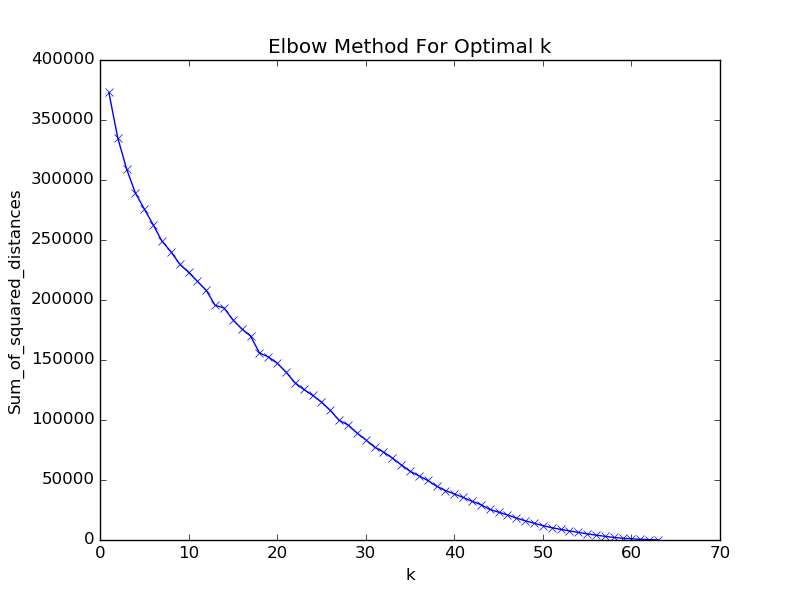
\includegraphics[width=\linewidth]{./figures/kmaxn.png}
	\caption{Optimal $k$ for maximum $k=n$}
   	\end{subfigure}
\end{figure} 
\begin{figure}[!htbp]
	\centering
   	\begin{subfigure}[!htbp]{0.7\linewidth}
    	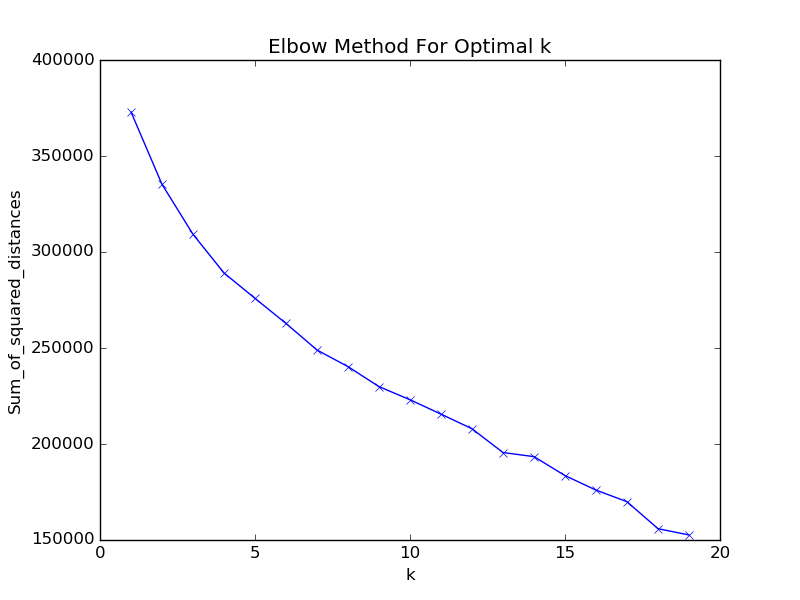
\includegraphics[width=\linewidth]{./figures/kmax20.png}
	\caption{Optimal $k$ for maximum $k=20$}
   	\end{subfigure}
\end{figure} 
\begin{figure}[!htbp]
	\centering
   	\begin{subfigure}[!htbp]{0.7\linewidth}
    	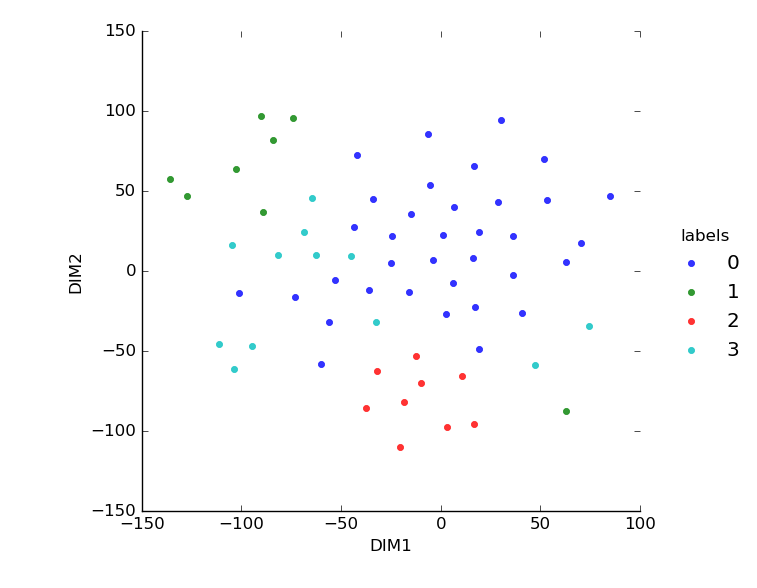
\includegraphics[width=\linewidth]{./figures/plot1.png}
	\caption{Optimal $k$ for maximum $k=20$}
   	\end{subfigure}
\end{figure} 


\end{document}






































